%% LyX 2.0.8.1 created this file.  For more info, see http://www.lyx.org/.
%% Do not edit unless you really know what you are doing.
\documentclass[english]{article}
\usepackage{ae,aecompl}
\usepackage{helvet}
\usepackage{beramono}
\renewcommand{\familydefault}{\rmdefault}
\usepackage[T1]{fontenc}
\usepackage{listings}
\usepackage{geometry}
\geometry{verbose,tmargin=2.5cm,bmargin=2.5cm,lmargin=2.5cm,rmargin=2.5cm,headheight=2.5cm,headsep=2.5cm,footskip=2.5cm}
\usepackage{amsmath}
\usepackage{amssymb}
\usepackage{graphicx}
\usepackage{setspace}
\onehalfspacing

\makeatletter
\AtBeginDocument{
  \def\labelitemii{\(\blacktriangleright\)}
  \def\labelitemiii{\(\blacksquare\)}
}

\makeatother

\usepackage{babel}
\begin{document}

\title{Software Implementation of Sailing Sea Monkey}


\author{CS13B027 Tirupati Hemanth Kumar\\
CS13B046 Aravind Krishna\\
CS13B062 Shreyas Harish}
\maketitle
\begin{abstract}
In the final part of assignment we implement the afore-mentioned block
cipher, optimized for \emph{X86 }architectures. The efficiency lies
in the fact that entire program of encryption($~$15 KB) and decryption
($~$15 KB) can entirely fit into $L_{1}$ caches of most modern day
machines.
\end{abstract}

\section*{Implementational Aspects of Ciphers}

The following are some software efficient techinques used for implementing
the cipher algorithm.
\begin{itemize}
\item Size of Executable:

\begin{itemize}
\item We have designed our implementation so that it can effectively fit
into few blocks of \emph{L1 }cache.
\item Inorder to achieve this, we computed T-tables for the proposed MDS
matrix. T-table construction for encryption and decryption are described
below.
\end{itemize}
\item Encryption T-table construction:

\begin{itemize}
\item Since the MDS matrix, $M=\left(\begin{array}{cc}
1 & 2\\
1 & 3
\end{array}\right)$, the encryption T-table would contain $a\Vert d$ and $2\times a\Vert3\times d$
values.
\item However storing $a\Vert d$ T-table is redundant since there is no
multiplication involved in this table(i.e, SBox outputs can be directly
used).$\implies$We only need to store a single T-table that contains
$2\times a\Vert3\times d$ values which has size of $512$ bytes.
\end{itemize}
\item Decryption T-table construction:

\begin{itemize}
\item Inverse MDS matrix is given by $M^{-1}=\left(\begin{array}{cc}
3 & 2\\
1 & 1
\end{array}\right)\implies$Decryption T-table must contain $3\times a\Vert b$ and $2\times a\Vert b$
values.
\item This would account for size of $512\times2\, bytes.$ On observing
that this is same as size of storing $2$ multiplication tables $(256\times2\, bytes)$
in $AES_{128}$ field, we can see that T-tables have space overhead
over storing multiplication tables. Hence, we directly used multiplication
tables of the field instead of T-tables incase of decryption.
\end{itemize}
\item Mode Of Operation:

\begin{itemize}
\item We use the cipher in Cipher Block Chain Mode so that low entropy information
can also be sent without loss of security.
\item For every encryption a new IV is generated using master key.
\item One disadvantage of using CBC mode is encryption would be done block
by block sequentially. This would add high performance overhead when
parallel encryption is desired. However we ignored this disadvantage
for simplistic software design.
\end{itemize}
\item We have also specifically avoided any key specific computations in
the implementation so that the executable run time does not have any
correlation with key used. 

\begin{itemize}
\item 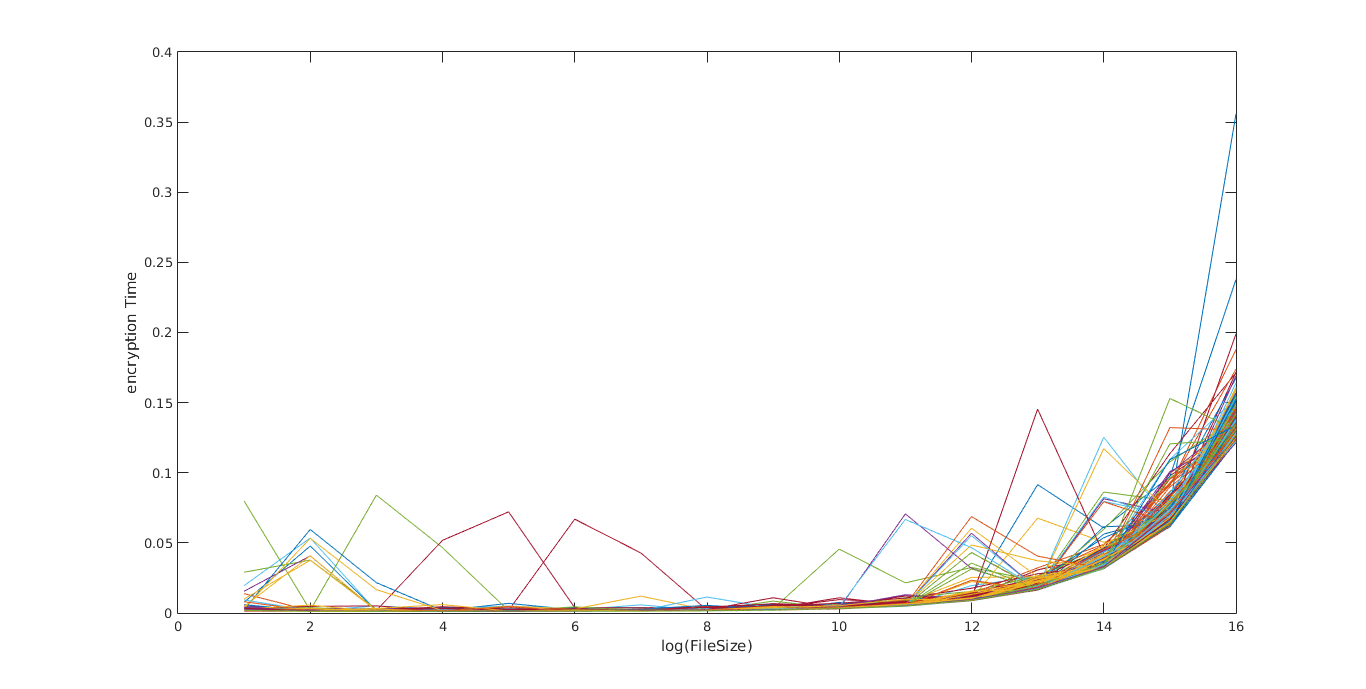
\includegraphics[scale=0.4]{timing}
\end{itemize}
\end{itemize}

\section*{Changes to Previous Submission}

While encryption algorithm itself is left unchanged, its mode of operation
is fixed as CBC.


\section*{Encryption time vs size of file}

The following graph depicts runtime of encryption and decryption on
various file sizes.

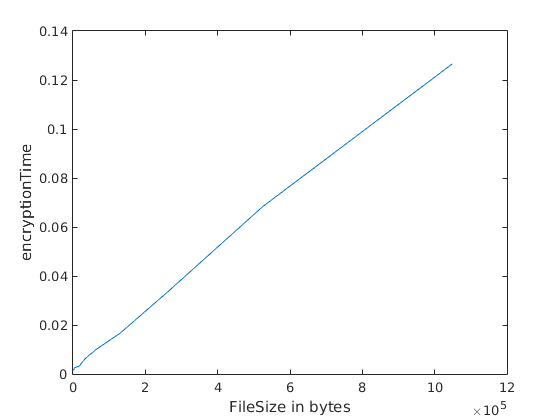
\includegraphics[scale=0.5]{untitled}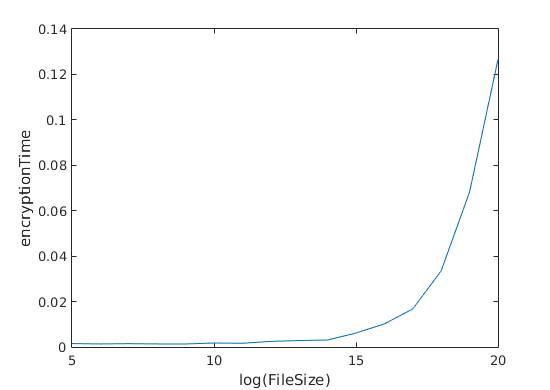
\includegraphics[scale=0.5]{untitled1}

We can see that run time of program is linear \emph{w.r.t }number
of bytes encrypted. This can attributed to CBC mode of operation which
encrypts the message block by block.


\section*{Working of the Cipher}

Working of cipher can verified using

\begin{lstlisting}[basicstyle={\ttfamily},numbers=right]
$ make enc
$ make encrypt
$ make dec
$ make decrypt
$ diff alice.txt alice.decrypt
$ 
\end{lstlisting}

\end{document}
